\usepackage{booktabs}%! Author = kyoto
%! Date = 08.03.2022


\section{Задание}
По выданному преподавателем варианту разработать программу асинхронного обмена данными с внешним устройством. При помощи
программы осуществить ввод или вывод информации, используя в качестве подтверждения данных сигнал (кнопку) готовности ВУ.


\begin{figure}[H]
    \centering
    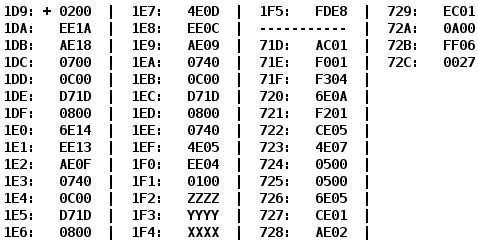
\includegraphics[scale=0.35]{img/variant}
\end{figure}


\section{Программа}

\subsection{Assembler}

\begin{center}
    \begin{tabular}{c}
        \begin{lstlisting}[basicstyle=\ttfamily]
        ORG     0x360
ADDR:	WORD	0x5A1
LEN:	WORD	0x0000
FIRST:	WORD	0x0000
SECOND: WORD    0x0000
START:  LD      (ADDR)+
        AND     #0xFF
        ST      LEN
L:      IN      7
        AND     #0x40
        BEQ     L
        LD      LEN
        OUT     6
BEGIN:	CLA
        LD      (ADDR)+
        ST      FIRST
        SWAB
        ST      SECOND
S1:     IN      7
        AND     #0x40
        BEQ     S1
        LD      FIRST
        OUT     6
        LOOP    LEN
        JUMP    S2
        JUMP    STOP
S2:     IN      7
        AND     #0x40
        BEQ     S2
        LD      SECOND
        OUT     6
        LOOP    LEN
        JUMP    BEGIN
STOP:	HLT

        \end{lstlisting}
    \end{tabular}
\end{center}

\newpage

\subsection{Описание программы:}
Вывод текста сохранённого в массиве в формате АДР0: ДЛИНА АДР1: СИМВ2 СИМВ1 АДР2: СИМВ4 СИМВ3 ... \\
\footnotesize (выводит сначала количество символов, а потом символы в порядке возрастания: СИМВ1, СИМВ2, СИМВ3)\\
\normalsize


\section{Область представления данных и область допустимых значений}

\subsection{Область представления:}
\noindentВ ячейке 360 беззнаковое 11тиразрядное 16теричное число (адрес ячейки).   \\
В ячейках 362-363 символ строки в кодировке ISO-8859-5. \\
В ячейке 361, 5A1 беззнаковое 8миразрядное 16теричное число.    \\
В дальнейших ячейках массива - беззнаковые 16теричные числа, с закодированными символами в младшем и старшем байте по одному в каждом. \\

\subsection{ОДЗ}

\subsubsection{ADDR:}
\begin{equation*}
    \begin{center}
        $0_{16} \leqslant ADDR \leqslant 7FF_{16}$\\
    \end{center}
\end{equation*}

\subsubsection{LEN:}
\begin{equation*}
    \begin{center}
        $0_{16} \leqslant LEN \leqslant FF_{16}$\\
        (на самом деле там одз нет, потому что мы выделяем маской значащие биты)
    \end{center}
\end{equation*}

\subsection{ADDR+LEN:}
\begin{equation*}
    \begin{center}
        \begin{cases}
            $0_{16} \leqslant ADDR+\frac{LEN}{2} \leqslant 360_{16}$ ,\\
            $382_{16} \leqslant ADDR+\frac{LEN}{2} \leqslant 7FF_{16}$\\
        \end{cases}
    \end{center}
\end{equation*}

\subsubsection{$M_i$:}
\begin{equation*}
    \begin{center}
        $20_{16} \leqslant $M_{i}$ \leqslant FF_{16}$\\
        (имеется ввиду ограничение на младший и старший байт элементов массива)
    \end{center}
\end{equation*}


\section{Расположение программы в памяти БЭВМ:}
\noindent\textit{Программы - \textbf{$360_{16}$-$381_{16}$} . \\
Выводимая строка – \textbf{5A1-(5A1+$\frac{LEN}{2}$-1)} .  \\}


\newpage


\section{Исполнение.}

\subsection{Выводимая строка:}
\begin{center}
    \begin{tabular}{|c|c|c|c|}
        \hline
        \textbf{Symbol} & \textbf{ISO-8859-5} & \textbf{UTF-8} & \textbf{UTF-16} \\
        \hline
        В               & 0xB2                & 0xD092         & 0x412           \\
        Е               & 0xB5                & 0xD095         & 0x415           \\
        Т               & 0xC2                & 0xD0A2         & 0x422           \\
        В               & 0xB2                & 0xD092         & 0x412           \\
        Ь               & 0xCC                & 0xD0AC         & 0x42С           \\
        \hline
    \end{tabular}
\end{center}

\subsection{Трассировка:}
\begin{center}
    \begin{tabular}{|l|l|l|l|l|l|r|l|l|r|r|l|l|}
        \toprule
        \textbf{Адр} & \textbf{Знач} & \textbf{IP} & \textbf{CR} & \textbf{AR} & \textbf{DR} & \textbf{SP} & \textbf{BR} & \textbf{AC} & \textbf{PS} & \textbf{NZVC} & \textbf{Адр} & \textbf{Знач} \\
        \midrule
        364          & AAFB          & 364         & 0           & 0           & 0           & 0           & 0           & 0           & 4           & 100           &              &               \\
        \hline
        364          & AAFB          & 365         & AAFB        & 5A1         & 5           & 0           & FFFB        & 5           & 0           & 0             & 360          & 05A2          \\
        \hline
        365          & 2FFF          & 366         & 2FFF        & 365         & FFFF        & 0           & FFFF        & 5           & 0           & 0             &              &               \\
        \hline
        366          & EEFA          & 367         & EEFA        & 361         & 5           & 0           & FFFA        & 5           & 0           & 0             & 361          & 5             \\
        \hline
        367          & 1207          & 368         & 1207        & 367         & 1207        & 0           & 367         & 40          & 4           & 100           &              &               \\
        \hline
        368          & 2F40          & 369         & 2F40        & 368         & 40          & 0           & 40          & 40          & 0           & 0             &              &               \\
        \hline
        369          & F0FD          & 36A         & F0FD        & 369         & F0FD        & 0           & 369         & 40          & 0           & 0             &              &               \\
        \hline
        36A          & AEF6          & 36B         & AEF6        & 361         & 5           & 0           & FFF6        & 5           & 0           & 0             &              &               \\
        \hline
        36B          & 1306          & 36C         & 1306        & 36B         & 1306        & 0           & 036B        & 5           & 0           & 0             &              &               \\
        \hline
        36C          & 200           & 36D         & 200         & 36C         & 200         & 0           & 036C        & 0           & 4           & 100           &              &               \\
        \hline
        36D          & AAF2          & 36E         & AAF2        & 5A2         & B2B5        & 0           & FFF2        & B2B5        & 8           & 1000          & 360          & 05A3          \\
        \hline
        36E          & EEF3          & 36F         & EEF3        & 362         & B2B5        & 0           & FFF3        & B2B5        & 8           & 1000          & 362          & B2B5          \\
        \hline
        36F          & 680           & 370         & 680         & 36F         & 680         & 0           & 036F        & B5B2        & 8           & 1000          &              &               \\
        \hline
        370          & EEF2          & 371         & EEF2        & 363         & B5B2        & 0           & FFF2        & B5B2        & 8           & 1000          & 363          & B5B2          \\
        \hline
        371          & 1207          & 372         & 1207        & 371         & 1207        & 0           & 371         & B540        & 8           & 1000          &              &               \\
        \hline
        372          & 2F40          & 373         & 2F40        & 372         & 40          & 0           & 40          & 40          & 0           & 0             &              &               \\
        \hline
        373          & F0FD          & 374         & F0FD        & 373         & F0FD        & 0           & 373         & 40          & 0           & 0             &              &               \\
        \hline
        374          & AEED          & 375         & AEED        & 362         & B2B5        & 0           & FFED        & B2B5        & 8           & 1000          &              &               \\
        \hline
        375          & 1306          & 376         & 1306        & 375         & 1306        & 0           & 375         & B2B5        & 8           & 1000          &              &               \\
        \hline
        376          & 8EEA          & 377         & 8EEA        & 361         & 4           & 0           & 3           & B2B5        & 8           & 1000          & 361          & 4             \\
        \hline
        377          & CE01          & 379         & CE01        & 377         & 379         & 0           & 1           & B2B5        & 8           & 1000          &              &               \\
        \hline
        379          & 1207          & 37A         & 1207        & 379         & 1207        & 0           & 379         & 40          & 4           & 100           &              &               \\
        \hline
        37A          & 2F40          & 37B         & 2F40        & 37A         & 40          & 0           & 40          & 40          & 0           & 0             &              &               \\
        \hline
        37B          & F0FD          & 37C         & F0FD        & 37B         & F0FD        & 0           & 037B        & 40          & 0           & 0             &              &               \\
        \hline
        37C          & AEE6          & 37D         & AEE6        & 363         & B5B2        & 0           & FFE6        & B5B2        & 8           & 1000          &              &               \\
        \hline
        37D          & 1306          & 37E         & 1306        & 37D         & 1306        & 0           & 037D        & B5B2        & 8           & 1000          &              &               \\
        \hline
        37E          & 8EE2          & 37F         & 8EE2        & 361         & 3           & 0           & 2           & B5B2        & 8           & 1000          & 361          & 3             \\
        \hline
        37F          & CEEC          & 36C         & CEEC        & 37F         & 036C        & 0           & FFEC        & B5B2        & 8           & 1000          &              &               \\
        \bottomrule
    \end{tabular}
\end{center}

\newpage

\begin{center}
    \centering
    \begin{tabular}{|l|l|l|l|l|l|r|l|l|r|r|l|l|}
        \toprule
        \textbf{Адр} & \textbf{Знач} & \textbf{IP} & \textbf{CR} & \textbf{AR} & \textbf{DR} & \textbf{SP} & \textbf{BR} & \textbf{AC} & \textbf{PS} & \textbf{NZVC} & \textbf{Адр} & \textbf{Знач} \\
        \midrule
        36C          & 200           & 36D         & 200         & 36C         & 200         & 0           & 036C        & 0           & 4           & 100           &              &               \\
        \hline
        36D          & AAF2          & 36E         & AAF2        & 5A3         & C2B2        & 0           & FFF2        & C2B2        & 8           & 1000          & 360          & 05A4          \\
        \hline
        36E          & EEF3          & 36F         & EEF3        & 362         & C2B2        & 0           & FFF3        & C2B2        & 8           & 1000          & 362          & C2B2          \\
        \hline
        36F          & 680           & 370         & 680         & 36F         & 680         & 0           & 036F        & B2C2        & 8           & 1000          &              &               \\
        \hline
        370          & EEF2          & 371         & EEF2        & 363         & B2C2        & 0           & FFF2        & B2C2        & 8           & 1000          & 363          & B2C2          \\
        \hline
        371          & 1207          & 372         & 1207        & 371         & 1207        & 0           & 371         & B240        & 8           & 1000          &              &               \\
        \hline
        372          & 2F40          & 373         & 2F40        & 372         & 40          & 0           & 40          & 40          & 0           & 0             &              &               \\
        \hline
        373          & F0FD          & 374         & F0FD        & 373         & F0FD        & 0           & 373         & 40          & 0           & 0             &              &               \\
        \hline
        374          & AEED          & 375         & AEED        & 362         & C2B2        & 0           & FFED        & C2B2        & 8           & 1000          &              &               \\
        \hline
        375          & 1306          & 376         & 1306        & 375         & 1306        & 0           & 375         & C2B2        & 8           & 1000          &              &               \\
        \hline
        376          & 8EEA          & 377         & 8EEA        & 361         & 2           & 0           & 1           & C2B2        & 8           & 1000          & 361          & 2             \\
        \hline
        377          & CE01          & 379         & CE01        & 377         & 379         & 0           & 1           & C2B2        & 8           & 1000          &              &               \\
        \hline
        379          & 1207          & 37A         & 1207        & 379         & 1207        & 0           & 379         & 40          & 4           & 100           &              &               \\
        \hline
        37A          & 2F40          & 37B         & 2F40        & 37A         & 40          & 0           & 40          & 40          & 0           & 0             &              &               \\
        \hline
        37B          & F0FD          & 37C         & F0FD        & 37B         & F0FD        & 0           & 037B        & 40          & 0           & 0             &              &               \\
        \hline
        37C          & AEE6          & 37D         & AEE6        & 363         & B2C2        & 0           & FFE6        & B2C2        & 8           & 1000          &              &               \\
        \hline
        37D          & 1306          & 37E         & 1306        & 37D         & 1306        & 0           & 037D        & B2C2        & 8           & 1000          &              &               \\
        \hline
        37E          & 8EE2          & 37F         & 8EE2        & 361         & 1           & 0           & 0           & B2C2        & 8           & 1000          & 361          & 1             \\
        \hline
        37F          & CEEC          & 36C         & CEEC        & 37F         & 036C        & 0           & FFEC        & B2C2        & 8           & 1000          &              &               \\
        \hline
        36C          & 200           & 36D         & 200         & 36C         & 200         & 0           & 036C        & 0           & 4           & 100           &              &               \\
        \hline
        36D          & AAF2          & 36E         & AAF2        & 5A4         & 00CC        & 0           & FFF2        & 00CC        & 0           & 0             & 360          & 05A5          \\
        \hline
        36E          & EEF3          & 36F         & EEF3        & 362         & 00CC        & 0           & FFF3        & 00CC        & 0           & 0             & 362          & 00CC          \\
        \hline
        36F          & 680           & 370         & 680         & 36F         & 680         & 0           & 036F        & CC00        & 8           & 1000          &              &               \\
        \hline
        370          & EEF2          & 371         & EEF2        & 363         & CC00        & 0           & FFF2        & CC00        & 8           & 1000          & 363          & CC00          \\
        \hline
        371          & 1207          & 372         & 1207        & 371         & 1207        & 0           & 371         & CC40        & 8           & 1000          &              &               \\
        \hline
        372          & 2F40          & 373         & 2F40        & 372         & 40          & 0           & 40          & 40          & 0           & 0             &              &               \\
        \hline
        373          & F0FD          & 374         & F0FD        & 373         & F0FD        & 0           & 373         & 40          & 0           & 0             &              &               \\
        \hline
        374          & AEED          & 375         & AEED        & 362         & 00CC        & 0           & FFED        & 00CC        & 0           & 0             &              &               \\
        \hline
        375          & 1306          & 376         & 1306        & 375         & 1306        & 0           & 375         & 00CC        & 0           & 0             &              &               \\
        \hline
        376          & 8EEA          & 378         & 8EEA        & 361         & 0           & 0           & FFFF        & 00CC        & 0           & 0             & 361          & 0             \\
        \hline
        378          & CE07          & 380         & CE07        & 378         & 380         & 0           & 7           & 00CC        & 0           & 0             &              &               \\
        \hline
        380          & 100           & 381         & 100         & 380         & 100         & 0           & 380         & 00CC        & 0           & 0             &              &               \\
        \bottomrule
    \end{tabular}
\end{center}
\newpage


\section{Доп. задание.}

\subsection{Задание:}
Ввод двух знаковых чисел с ВУ-9 (цифровая клавиатура), вывод максимального из них на ВУ-2

\begin{center}
    \begin{tabular}{c}
        \begin{lstlisting}[basicstyle=\ttfamily\tiny]
            ORG     0x0
NUM1:	    WORD	0x0
NUM2:	    WORD	0x0
X:	        WORD	0x0
SYMBOL:     WORD    0x0
FLAG:       WORD    0x0
START:      CALL    $INIT
FIRST:      CLA
            CALL    $READ
            CALL    $SIGNFLAG
            LD      $FLAG
            BNE     CYCLE
            LD      $SYMBOL
            ST      $X
CYCLE:      CALL    $READ
            CALL    $SEPCHECK
            CALL    $ENDCHECK
            CALL    $SAVE
            JUMP    $CYCLE
FINAL:      LD      $NUM1
            CMP     $NUM2
            BMI     N2
            PUSH
            CALL    $SOUT
            POP
            JUMP    $STOP
N2:         LD      $NUM2
            PUSH
            CALL    $SOUT
            POP
            JUMP    $STOP
SOUT:       IN      0x7
            AND     #0x40
            BEQ     SOUT
            LD      (SP+1)
            OUT     0x6
            RET
STOP:       HLT
INIT:       ST    $NUM1
            ST    $NUM2
            ST    $X
            ST    $SYMBOL
            ST    $FLAG
            RET
READ:       IN    0x1D
            AND   #0x40
            BEQ   READ
            IN    0x1C
            ST    $SYMBOL
SIGNFLAG:   LD      $SYMBOL
            CMP     #0xA
            BNE     FRET
            LD      #0x1
            ST      $FLAG
FRET:       RET
SEPCHECK:   LD  $SYMBOL
            CMP     #0xC
            BNE     SEPRET
            LD      $X
            PUSH
            CALL    $SIGN
            POP
            ST      $NUM1
            POP
            JUMP    $FIRST
SEPRET:     RET
ENDCHECK:   LD  $SYMBOL
            CMP     #0xF
            BNE     ERET
            LD      $X
            PUSH
            CALL    $SIGN
            POP
            ST      $NUM2
            POP
            JUMP    $FINAL
ERET:       RET
SAVE:       LD     $X
            ADD    $X
            ADD    $X
            ADD    $X
            ADD    $X
            ADD    $X
            ADD    $X
            ADD    $X
            ADD    $X
            ADD    $X
            ADD    $SYMBOL
            ST     $X
            RET
SIGN:       LD     $FLAG
            BEQ    STX
            LD     (SP+1)
            NEG
            ST     (SP+1)
            CLA
            ST     $FLAG
STX:        ST     $X
            RET
        \end{lstlisting}
    \end{tabular}
\end{center}